\chapter{Thermal physics}
\section{Heat transfer}
\begin{definition}{Thermal equilibrium}{thermal-eq}
	The phenomenon in which two bodies in thermal contact
	have \it{no net exchange of heat} between them.
\end{definition}
\begin{definition}{0LoT}{0lot}
	If bodies A and B are \it{separately in thermal eq.}~with a third body
	C, then A and B are in thermal eq.~with each other.
\end{definition}
\begin{definition}{Heat capacities}{heat-capacity}
	\par
	\bf{Specific heat capacity} \(c\) is the amount of energy
	per unit mass required to cause an increase in one unit of temperature [\unit{\joule\per\kilogram\per\kelvin}].
	\[Q=mc\Delta T\]

	\bf{Heat capacity} \(C\) is the amount of energy
	required to cause an increase in one unit of temperature [\unit{\joule\per\kelvin}].
	\[Q=C\Delta T\]
\end{definition}
\begin{definition}{Latent heats}{latent-heat}
	\par
	\bf{Specific latent heat of fusion} \(l_f\) --- the amount of energy
	per unit mass required to change a substance \it{from solid to liquid} with no change in temperature [\unit{\joule\per\kilogram}].
	\[Q=ml_f\]

	\bf{Specific latent heat of vaporization} \(l_v\) --- the amount of energy
	per unit mass required to change a substance \it{from liquid to gas} with no change in temperature [\unit{\joule\per\kilogram}].
	\[Q=ml_v\]
\end{definition}

Solving problems involving heat transfer involve \term{energy conservation}.
\[\text{total heat loss} = \text{total heat gain}\]

\begin{example}{}{ct1-q7}
	A glass beaker (\(m_b = \qty{170}{\gram}\), \(c_b = \qty{0.84}{\joule\per\gram\per\kelvin}\))
	at \qty{28}{\celsius} contains \it{ice} (\(m_i = \qty{120}{\gram}\), \(c_i=\qty{2.05}{\joule\per\gram\per\kelvin}\))
	at \qty{-15}{\celsius} and boiling \it{water} (\(m_w = \qty{90}{\gram}\), \(c_w = \qty{4.18}{\joule\per\gram\per\kelvin}\)).

	When thermal equilibrium is reached, there is both water and ice in the beaker. No water evaporates.
	(\(l_f = \qty{334}{\joule\per\gram}\))

	\it{Find the mass of ice \({m_i}'\) that melts during this process.}
	\vspace*{5mm}

	deduction---
	\begin{center}
		`water and ice in the beaker' \(\implies\) final temperature is \qty{0}{\celsius} \\
		`thermal equilibrium reached' \(\implies\) heat lost = heat gained; final temperature is the same for all bodies
	\end{center}
	\vspace*{5mm}

	working---
	\begin{align*}
		\sum\text{heat loss}                  & = \sum\text{heat gain}                \\
		m_w c_w\ab(100-0)  + m_b c_b\ab(28-0) & = m_i c_i\ab(0-\ab(-15)) + {m_i}' l_f \\
		{m_i}'                                & = \qty{114}{\gram}
	\end{align*}
\end{example}

\section{Molecular view}
\begin{definition}{Internal energy}{internal-energy}
	The summation of:
	\begin{itemize}
		\item \it{microscopic kinetic energy} due to the molecules' random motion
		\item \it{microscopic potential energy} due to intermolecular forces
	\end{itemize}
	\[U = \sum E_k + \sum E_p\]
\end{definition}
\begin{definition}{Temperature}{temperature}
	A measure of the average kinetic energy of the molecules in a substance.
\end{definition}
\begin{table}[htpb]
	\centering
	\begin{tabular}{r c c}
		\toprule
		                        & \(E_k\)           & \(E_p\) \\
		\midrule
		phase change            & ---               & change  \\
		\(T\) increase/decrease & increase/decrease & ---     \\
		\bottomrule
	\end{tabular}
	\label{tab:ek-ep}
	\caption{What changes?}
\end{table}

\section{Ideal gases}
\begin{definition}{Ideal gas}{ideal-gas}
	A theoretical model of a gas which satisfies
	\[pV = nRT\]
	where \(p\) is the pressure, \(V\) is the volume, \(n\) is the number of moles, \(R\) is the ideal gas constant and \(T\) is the temperature.
\end{definition}
Ideal gas \bf{assumptions} include
\begin{itemize}
	\item A gas consists of a very large number of molecules
	\item The molecules are in constant random motion
	\item Gas molecules' collisions with one another and the container walls are perfectly elastic
	\item No intermolecular forces between gas molecules
	\item Volume of gas molecules is negligible compared to the volume of the container
	\item Duration of collisions is negligible compared to the time between collisions
\end{itemize}
\subsection{Pressure}
\begin{definition}{Gas pressure}{gas-pressure}
	The \it{average force per unit area} exerted by gas molecules on the container walls
\end{definition}
Pressure is due to number of molecules \(N\), molecule mass \(m\), molecule speed \(c\) and volume \(V\).

Assume a large number of molecules \(N\) in a cubical container of side \(s\).
For each molecule, resolve its velocity \(c_i\) in 3d; \({c_i}^2 = {u_i}^2 + {v_i}^2 + {w_i}^2\).

Choose any container wall. In the \(x\)-direction, a molecule colliding with the wall
will experience a change in momentum
\[\Delta p = p_f-p_i = -mu-\ab(+mu) = -2mu\]

The time taken for any collision \(\Delta t = \f{2s}{u}\), so the average force exerted
on the chosen wall by one molecule is
\[\ab<F> = \ab|\f{\Delta p}{\Delta t}| = \f{2mu\cdot u}{2s} = \f{mu^2}{s}\]

The total force exerted on the wall by all \(N\) molecules is
\[\sum F = N\ab<F> = \f{Nm\ab<u^2>}{s}\]

The total pressure exerted on the wall is the total force per unit area:
\[p = \f{\sum F}{s^2} = \f{Nm\ab<u^2>}{s^3} = \f{Nm\ab<u^2>}{V}\]

Given that \(\ab<c^2> = \ab<u^2> + \ab<v^2> + \ab<w^2>\), and
because all molecules are in constant random motion (with no preferred direction),
\[\ab<u^2> = \f{1}{3}\ab<c^2>\]
Thus
\begin{equation*}
	pV = \f{1}{3}Nm\ab<c^2>
\end{equation*}
\(\ab<c^2>\) is the mean square speed; \(\sqrt{\ab<c^2>}\) is the r.m.s.~speed.

\subsection{Temperature}
Derive:
\begin{align*}
	pV = \f{1}{3}Nm\ab<c^2>               & = NkT                        \\
	\implies \f{1}{2}m\ab<c^2>            & = \f{3}{2}kT                 \\
	\implies U =  N\cdot\f{1}{2}m\ab<c^2> & = \f{3}{2}NkT  = \f{3}{2}nRT \\
\end{align*}
The internal energy is directly proportional to the temperature (\(U\propto T\))\sidenote{assuming gas is monoatomic}; it is independent of the pressure and volume.

\section{State}
\begin{definition}{1LoT}{1lot}
	The increase in internal energy of a system is equal to
	the (1) \it{heat supplied to the system} plus the (2) \it{work done \bf{on the system}} by external forces.
	\[\Delta U = Q + W\]
	\small \[W = \int p\odif{V}\]
\end{definition}
\begin{table}[htpb]
	\centering
	\begin{tabular}{r c c}
		\toprule
		      & \(Q\)              & \(W\)            \\
		\midrule
		\(+\) & heat enters system & system contracts \\
		\(-\) & heat leaves system & system expands   \\
		\bottomrule
	\end{tabular}
	\label{tab:q-and-w}
	\caption{Signs of \(Q\) and \(W\)}
\end{table}

Some important thermodynamic processes\sidenote{we defined \(W\) as `work done on the system', so \(\Delta V>0\implies W<0\) and v.v.}:
\begin{table}[htpb]
	\centering
	\begin{tabular}{r l c c c}
		\toprule
		process       & involves         & \(Q =\)        & \(W=\)              & \(\Delta U=\) \\
		\midrule
		isothermal    & \(T\) constant   & \(-W\)         & \(-\int p\odif{V}\) & \(0\)         \\
		isovolumetric & \(V\) constant   & \(mc\Delta T\) & \(0\)               & \(Q\)         \\
		adiabatic     & no heat transfer & \(0\)          & \(-\int p\odif{V}\) & \(W\)         \\
		isobaric      & \(p\) constant   & \(mc\Delta T\) & \(-p\Delta V\)      & \(Q+W\)       \\
		\bottomrule
	\end{tabular}
	\caption{Thermodynamic processes}
	\label{tab:thermo-processes}
\end{table}

\begin{marginfigure}
	\centering
	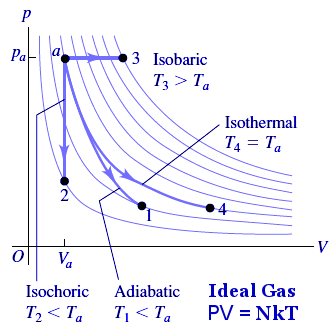
\includegraphics[width=\textwidth]{assets/thermo-processes.png}
	\caption{\(pV\) diagrams}
	\label{fig:pv-diagram}
\end{marginfigure}

\begin{definition}{Cyclic process}{cyclic-process}
	A process in which the system returns to its initial state at the end of the process.
	\[\Delta U = 0 \implies Q_\text{net} = -W_\text{net}\]
\end{definition}
